\documentclass[12pt,a4paper,twoside,titlepage,openright]{report}

\usepackage[utf8]{inputenc}
\usepackage{amsmath}
\usepackage{amsfonts}
\usepackage{amssymb}
\usepackage{lmodern}
\usepackage{setspace}
\usepackage{siunitx}
\usepackage{titlesec}
\usepackage{graphicx}
\usepackage{tabularx}
\usepackage{geometry}
\usepackage{subfig}
\usepackage[subfigure]{tocloft}
\usepackage{fancyhdr}
\usepackage[english]{babel}
\usepackage{blindtext}
\usepackage{hyperref}

% do not display the chapter-headings
\titleformat{\chapter}[display]
  {\normalfont\huge\bfseries}{}{0pt}{\Huge}
 
% reference figures, sections and equations
\newcommand{\figref}[1]{{(Figure \ref{#1})}}
\newcommand{\secref}[1]{{(Section \ref{#1})}}
\newcommand{\neweqref}[1]{{(Equation \ref{#1})}}

% list of equations
\newcommand{\listequationsname}{List of Equations}
\newlistof{equationname}{equ}{\listequationsname}
\newcommand{\equationname}[1]{%
\addcontentsline{equ}{figure}{\protect\numberline{\theequation} #1}\par}
 
% create an completely empty page
\newcommand{\emptypage}
{
	\newpage
	\thispagestyle{empty}
	\mbox{}
}

\begin{document}	
	% page numbers left and right on even and odd pages
	\fancypagestyle{plain}
	{
		\fancyhf{}
		\renewcommand{\headrulewidth}{0pt}
		\renewcommand{\footrulewidth}{0.4pt}
		\fancyfoot[LE]{\thepage}
		\fancyfoot[RO]{\thepage}
	}
	\pagestyle{fancy}
	\fancyhf{}
	\renewcommand{\headrulewidth}{0pt}
	\renewcommand{\footrulewidth}{0.4pt}
	\fancyfoot[LE]{\thepage}
	\fancyfoot[RO]{\thepage}
	
	\begin{titlepage}
	\newgeometry{top=1in,bottom=1in,right=1in,left=1in}
	
	\begin{flushleft}
		\begin{tabularx}{\linewidth}{@{}llXr@{}}
			
\includegraphics[height=1.5cm]{figures/ei_logo.pdf} &	
			
\includegraphics[height=1.5cm]{figures/hsa_logo.pdf} & 
			& 
			
\includegraphics[height=1.5cm]{figures/tum_logo.pdf}
		\end{tabularx}
	\end{flushleft}
	\hfill \\[1cm]
	
	\begin{flushleft}
		Technische Universität München \\
		Department of Electrical Engineering and Information Technology \\
		Institute of Power Transmission Systems \\[4cm]
	\end{flushleft}
		
	\begin{center}
		\huge
		Implementation and Evaluation of the Holomorphic Embedding Load Flow Method\\[1cm]
		\large
		Benedikt Schmidt, B.Sc. \\
		\textit{benedikt.schmidt@tum.de} \\[7cm]
	\end{center}
	
	\begin{flushleft}
		Supervisor: Markus Meyer, M.Sc. \\
		Supervising Professor: Prof. Dr.-Ing. Rolf Witzmann \\
		Date of submission: 31.03.2015
	\end{flushleft}
\end{titlepage}
	
	% the title page set a different layout
	\newgeometry{top=1in,bottom=1in,right=1in,left=2in}
	
	\emptypage
	\begin{abstract}
A load-flow calculation is a key element in planning and running power nets. During the past centuries only iterative methods with insufficient convergence behaviour were available for this task. Recent research resulted in a new approach for this problem, the so-called \emph{Holomorphic Embedding Load Flow} (\emph{HELM}). During this thesis I will explain how this method can be applied and compare it to the iterative methods. I will show that the superior convergence behaviour of \emph{HELM} enables the load-flow calculation of nets closer to their border of stability than with iterative methods. This is reached by a trade-off with respect to runtime; therefore, in practice one has to evaluate the use of \emph{HELM}.
\end{abstract}
	
	% ensure that the page number is the identical with the pdf page number
	\setcounter{page}{4}

	\emptypage
	\tableofcontents
	
	\chapter{Introduction}
The energy revolution, driven by consumers, politics and the society at whole, is stressing our power supply system. For instance, the decision to shut down the atomic power plants in Germany in the foreseeable future will shift the main power sources from the South of Germany into the North. Historically, these sources were placed close to the main loads in the power net, but with the need to use renewable energy sources our power plants will be located where these energy sources are available and not where the big cities and the industry was built. Therefore, our power nets will have to change to be able to transport the energy from the sources to the loads.

One of the necessary steps for a change in the power net is a static load-flow calculation, for which only algorithms with a bad convergence behaviour during the past were available. These algorithms have one thing in common: they are iterative and can therefore not guarantee to find the physical correct solution. With this drawback in mind, a totally new approach called \emph{Holomorphic Embedding Load Flow} (\emph{HELM})  \citep{helmIEEE} was developed by Antonio Trias, described more detailed in \secinref{helm}. This approach guarantees to find a solution for a given load-flow problem if, and only if, the system is stable. Unfortunately, this method is so far only implemented in \emph{HELM-Flow} \footnote{http://www.gridquant.com/solutions/helm-flow/} by Gridquant. The in europe common tool \emph{PSS SINCAL} \footnote{http://www.simtec.cc/sites/sincal.asp} has not yet implemented this new approach, but it is the tool of choice for instance at the Institute of Power Transmission Systems at the Technische Universität München. Therefore, I implemented a tool which can apply \emph{HELM} to a power net stored in the file format of \emph{PSS SINCAL}.

The main results of this thesis are:
\begin{itemize}
	\item \emph{HELM} has a better convergence behaviour than the iterative methods.
	\item The theoretical perfect behaviour of \emph{HELM} can only be reached through a trade-off with respect to runtime.
\end{itemize}	
	\chapter{Load-Flow Calculation}

\section{Problem Formulation}
The aim of an load-flow analysis is to determine the voltages in the power net. Any further information, like currents in connections, critically low voltages, etc. can be derived from this result. Therefore I will consider the problem to be solved if the voltages are known.

The first step in a load flow analysis is the modelling of the net elements, as it is way to complex to use a detailed description of for instance a power plant like \figref{power_plant}. Therefore, all elements in a power net are modelled through busses, also called nodes, and admittances between them. To simplify the calculations only single phase nets are considered, therefore three phase systems have to scaled down by the factor 3, respective $\sqrt{3}$. In the model also exists only one voltage level, which means that all admittances, powers and voltages have to be scaled according to this.

The second step is then the actual calculation of the node voltages, which based is on a nodal analysis. As a pure nodal analysis is only capable of current loads it is extended to support more realistic load models.

\begin{figure}
	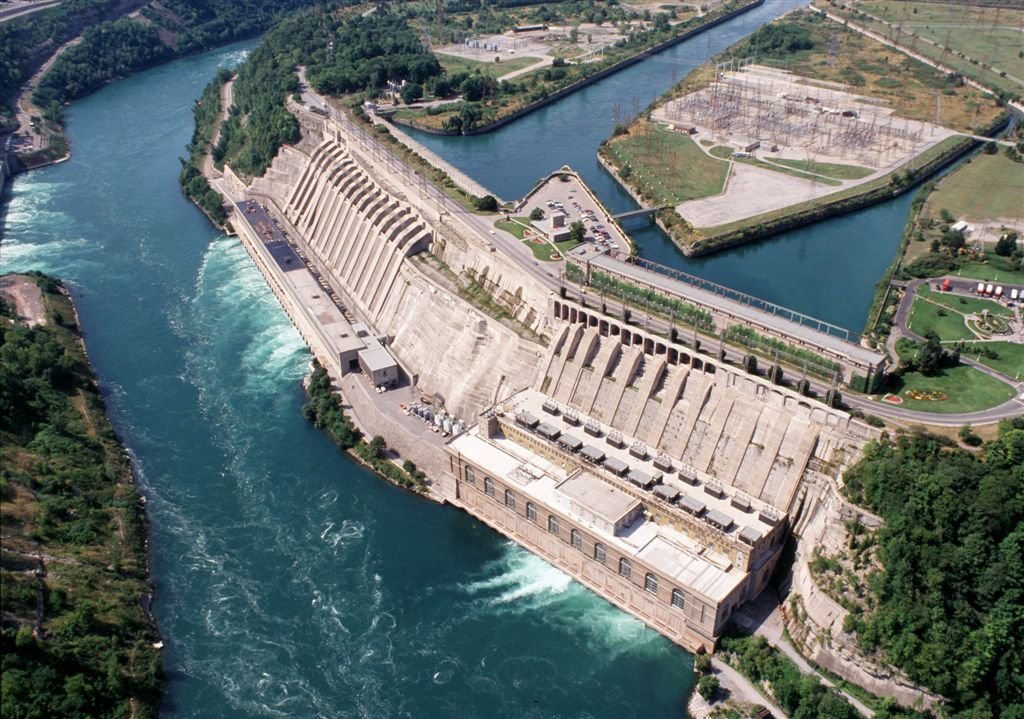
\includegraphics[width=\textwidth]{figures/adam_beck_complex.jpg}
	\caption{Sir Adam Beck Hydroelectric Generating Stations \citep{adam_back_complex}}
	\label{fig:power_plant}
\end{figure}

\subsection{Busses}
The most basic mathematical description of a an electric circuit, which an power net is, would be through admittances $Y_{ik}$ between the nodes $i$ and $k$, node voltages $U_k$ and branch currents $I_k$. In this case the element-based formulation
\begin{equation}
	\sum_i Y_{ik} U_i = I_k,
	\label{eq:current_controlled}
\end{equation}
will be used. If the loads and inputs would be current-controlled we could already stop at this point, solve the equation system and receive the node voltages as result. Unfortunately, most elements in a power net are defined through power, which is fed in, and load, which is drawn from the power net. Therefore, we have to extend \neweqref{current_controlled} with a term for a constant power $S_k = P_k + j Q_k = U_k I_k^\star$ at the node $k$ and receive
\begin{equation}
	\sum_i Y_{ik} U_i = I_k + \frac{S_j^\star}{U_j^\star}.
	\label{eq:pq_bus}
\end{equation}
This formula is already the definition of a so-called PQ-bus, as at the node the real and reactive power is the defined.
Another type of bus is a slack bus. At this bus the voltage is defined, therefore we do not need any further description of this bus, but the bus is also part from neighbour busses through the branch currents $Y_{ik} U_i$. In this case, if one of the branch currents is already known, this value can be moved to the right hand side of the equation \neweqref{pq_bus} and combined with $I_k$. Although, slack busses show up only in the constant currents of the right hand sides, there must be always at least one slack bus in the power net, as this bus then defines the rotation of the system and compensates mismatches in the total power sum. In practice, typically a major power plant is selected as slack bus.
The third important type of bus, beside the slack bus and PQ-bus, is the PV-bus. This is already some sort of control, as at such a node the real power $P_k$ and the voltage magnitude $|U_k|$ is defined. The implementation of this bus type depends on the algorithm which is used to calculate the missing node voltages, therefore I will discuss this in the section about the algorithms.

\subsection{Admittance Matrix}
The admittance matrix $\mat Y = (Y_{ik})$ is filled with the admittances between the nodes. More complex elements, like controlled sources, actually have to be voltage controlled, so that they can be modelled with an admittance matrix. Fortunately, most elements, which are not voltage controlled, can be transformed through a gyrator, which itself can be modelled through voltage controlled elements.

As during the modelling later several kinds of electric elements are used I will describe for each of them how they effect the admittance matrix. Each circuit element is there defined through a partial admittance matrix $\mat Y_p$, which have to be summed up afterwards to get the total admittance matrix $\mat Y$:
\begin{equation}
	\mat Y = \sum_i \mat Y_{p,i}
\end{equation}

The same superposition applies also for the current sources, if there are any.
\begin{equation}
	\vec I = \sum_i \vec I_{p,i}
\end{equation}

The two most important elements are the admittance, which is part of nearly every model of a net element, and the ideal transformer, which is mainly used for modelling real transformers which non-nominal ratios. The controlled source and the gyrator are actually only used to model the ideal transformer, which is build upon these elements.

\subsubsection{Admittance}

\begin{figure}
	\centering
	\begin{circuitikz}
	\draw (0, 0) node[left] {$U_\alpha$} to [R=$G$,o-o] (3, 0) node[right] {$U_\beta$};
\end{circuitikz} 

	\caption{Admittance $G$ between the nodes $\alpha$ and $\beta$}
	\label{fig:admittance}
\end{figure}

The admittance $G$ between the nodes $\alpha$ and $\beta$ \figref{admittance} causes the currents
\begin{equation}
	I_\alpha = (U_{k,\alpha} - U_{k,\beta}) G
\end{equation}
and
\begin{equation}
	I_\beta = (U_{k,\beta} - U_{k,\alpha}) G,
\end{equation}
which have to be considered in the admittance matrix through
\begin{equation}
	\mat Y_p = 	
	\begin{blockarray}{cccccc}
		\begin{block}{[ccccc]c}
		 		& \vdots	&			& \vdots	&			& \\
		\cdots	& G			& \cdots	& -G		& \cdots	& \alpha \\
		 		& \vdots	&			& \vdots	&			& \\
		\cdots	& -G		& \cdots	& G			& \cdots	& \beta \\
		 		& \vdots	&			& \vdots	&			& \\
		\end{block}
				& \alpha	&			& \beta		&			& 
	\end{blockarray}
\end{equation}

\subsubsection{Voltage Controlled Current Source}

\begin{figure}
	\centering
	\begin{circuitikz}
	\draw (0, 0) node[left] {$U_\delta$} to[open,o-o,v^=$u_{in}$] (0, 4) node[left] {$U_\gamma$};
	\draw (3, 4) to[european controlled current source,i=$g_m u_{in}$] (3, 0);
	\draw (3, 4) to[short,-o] (4, 4) node[right] {$U_\alpha$};
	\draw (3, 0) to[short,-o] (4, 0) node[right] {$U_\beta$};
\end{circuitikz} 

	\caption{Voltage controlled current source}
	\label{fig:voltage_controlled_current_source}
\end{figure}

The voltage controlled current source (VCCS) is again defined through the two branch currents
\begin{equation}
	I_\alpha = (U_{k,\gamma} - U_{k,\delta}) g_m
\end{equation}
and
\begin{equation}
	I_\beta = (U_{k,\delta} - U_{k,\gamma}) g_m,
\end{equation}
but with the difference to the admittance that this time the current is controlled by different nodes.

\begin{equation}
	\mat Y_p = 	
	\begin{blockarray}{cccccc}
		\begin{block}{[ccccc]c}
		 		& \vdots	&			& \vdots	&			& \\
		\cdots	& g_m		& \cdots	& -g_m		& \cdots	& \alpha \\
		 		& \vdots	&			& \vdots	&			& \\
		\cdots	& -g_m		& \cdots	& g_m		& \cdots	& \beta \\
		 		& \vdots	&			& \vdots	&			& \\
		\end{block}
				& \gamma	&			& \delta	&			& 
	\end{blockarray}
\end{equation}

\subsubsection{Gyrator}

\begin{figure}
	\centering
	\begin{circuitikz}
	\draw (0, 0) node[gyrator] (G) {};
	\draw (G.base) node{$G_D$};
  	\draw ($(G.A1) - (1, 0)$) node[left] {$U_\alpha$} to[short,o-,i=$i_1$] (G.A1);
  	\draw (G.A2) to[short,-o] ($(G.A2) - (1, 0)$) node[left] {$U_\beta$};
  	\draw ($(G.B1) + (1, 0)$) node[right] {$U_\gamma$} to[short,o-,i=$i_2$] (G.B1);
  	\draw (G.B2) to[short,-o] ($(G.B2) + (1, 0)$) node[right] {$U_\delta$};
  	\draw ($(G.A2) - (1, 0)$) to[open,v^=$u_1$] ($(G.A1) - (1, 0)$);
  	\draw ($(G.B2) + (1, 0)$) to[open,v=$u_2$] ($(G.B1) + (1, 0)$);
\end{circuitikz}
	\caption{Gyrator}
	\label{fig:gyrator_original}
\end{figure}

\begin{figure}
	\centering
	\begin{circuitikz}	
	\draw (1, 2.5) to[european controlled current source,i_=$G_D u_2$] (1, 0);
	\draw (-1, 2.5) node[left] {$U_\alpha$} to[short,i=$i_1$,o-] (1, 2.5);
	\draw (1, 0) to[short,-o] (-1, 0) node[left] {$U_\beta$};
	\draw (-1, 0) to[open,v^=$u_1$] (-1, 2.5);
	\draw (3, 2.5) to[european controlled current source,i=$-G_D u_1$] (3, 0);
	\draw (5, 2.5) node[right] {$U_\gamma$} to[short,i=$i_2$,o-] (3, 2.5);
	\draw (3, 0) to[short,-o] (5, 0) node[right] {$U_\delta$};
	\draw (5, 0) to[open,v=$u_2$] (5, 2.5);
\end{circuitikz} 

	\caption{Equivalent circuit for a gyrator}
	\label{fig:gyrator_equivalent}
\end{figure}

The gyrator \figref{gyrator_original}, which is defined by
\begin{equation}
	i_1 = G_D u_2
\end{equation}
and
\begin{equation}
	i_2 = -G_D u_1
\end{equation}
can be replaced with two VCCSs like in \figref{gyrator_equivalent}.

\subsubsection{Ideal Transformer}

\begin{figure}
	\centering
	\begin{circuitikz}
	\draw (0, 0) node[transformer core] (T) {};
	\draw ($(T.base) + (0, 0.3)$) node{$a : 1$};
  	\draw ($(T.A1) - (1, 0)$) node[left] {$U_\alpha$} to[short,o-,i=$i_1$] (T.A1);
  	\draw (T.A2) to[short,-o] ($(T.A2) - (1, 0)$) node[left] {$U_\beta$};
  	\draw ($(T.B1) + (1, 0)$) node[right] {$U_\gamma$} to[short,o-,i=$i_2$] (T.B1);
  	\draw (T.B2) to[short,-o] ($(T.B2) + (1, 0)$) node[right] {$U_\delta$};
  	\draw ($(T.A2) - (1, 0)$) to[open,v^=$u_1$] ($(T.A1) - (1, 0)$);
  	\draw ($(T.B2) + (1, 0)$) to[open,v=$u_2$] ($(T.B1) + (1, 0)$);
\end{circuitikz}
	\caption{Ideal transformer}
	\label{fig:ideal_transformer_original}
\end{figure}

\begin{figure}
	\centering
	\begin{circuitikz}
	\draw (0, 0) node[gyrator] (G1) {};
	\draw (2, 0) node[gyrator] (G2) {};
	\draw (G1.base) node{$a R$};
	\draw (G2.base) node{$R$};
	\draw (G1.B1) to[short,-*] (G1.B1) node[above] {$U_\epsilon$};
  	\draw ($(G1.A1) - (0.5, 0)$) node[left] {$U_\alpha$} to[short,o-,i=$i_1$] (G1.A1);
  	\draw (G1.A2) to[short,-o] ($(G1.A2) - (0.5, 0)$) node[left] {$U_\beta$};
  	\draw ($(G2.B1) + (0.5, 0)$) node[right] {$U_\gamma$} to[short,o-,i=$i_2$] (G2.B1);
  	\draw (G2.B2) to[short,-o] ($(G2.B2) + (0.5, 0)$) node[right] {$U_\delta$};
  	\draw ($(G1.A2) - (0.5, 0)$) to[open,v^=$u_1$] ($(G1.A1) - (0.5, 0)$);
  	\draw ($(G2.B2) + (0.5, 0)$) to[open,v=$u_2$] ($(G2.B1) + (0.5, 0)$);
  	\draw (G1.A2) to[short] (G1.B2);
\end{circuitikz}
	\caption{Equivalent circuit for an ideal transformer}
	\label{fig:ideal_transformer_equivalent}
\end{figure}

An ideal transformer like in \figref{ideal_transformer_original} is modelled with two gyrators according to the circuit \figref{ideal_transformer_equivalent}. The gyrators themselves have to be replaced by voltage controlled elements, like it was presented previously.

The parameter $R$ in this model can be chosen freely in theory, but for numerical reasons I recommend such a scaling of the internal node, that it is in the range of the nominal voltages. To be able to do this an estimation of the load flow over the transformer is needed, but it is sufficient to have a very rough estimate. If the scaling is chosen improperly especially the iterative methods to solve the load flow problem will not convergence in most cases.

\section{Scaling}
As long as the relations are kept the same it is possible to change the scale base of all values in a system. For purpose from the set of voltage, current, impedance and power two physical quantities can be freely chosen and the others arise out of this decision. Another term for this scaling is the transformation into a so-called per-unit system \citep[p. 90]{powerSystemAnalysis}.

For numerical stability the voltages should be in the range of 1, therefore for each voltage level in the system the nominal voltage is selected as scale base $U_B$ for the voltages. The degree of freedom can be used to scale also the powers down into the range of 1, which can be achieved for instance roughly with the scale base
\begin{equation}
	P_B = \frac{1}{2n} \left( \sum_{i}^n \left| P_{load,i} \right| + \sum_{i}^n \left| Q_{load,i} \right| \right)
\end{equation}
for the powers. 

The other scale bases are then derived from these two chosen values:
\begin{equation}
	I_B = \frac{P_B}{U_B}
\end{equation}
\begin{equation}
	Z_B = \frac{1}{Y_B} = \frac{U_B}{I_B}
\end{equation}

The actually scaling is achieved through a division of the values by the scale bases.
\begin{equation}
	U_{scaled} = \frac{U}{U_B}
\end{equation}
\begin{equation}
	I_{scaled} = \frac{I}{I_B}
\end{equation}
\begin{equation}
	P_{scaled} = \frac{P}{P_B}
\end{equation}
\begin{equation}
	Q_{scaled} = \frac{Q}{P_B}
\end{equation}
\begin{equation}
	Z_{scaled} = \frac{Z}{Z_B}
\end{equation}
\begin{equation}
	Y_{scaled} = \frac{Y}{Y_B}
\end{equation}

\section{Modelling of Net Elements}

The power net elements are modelled through admittances and busses, therefore we will use the previously derived knowledge to describe the behaviour of the net elements.

All external nodes which exist in a power net are by default PQ-busses with no load, therefore $P = 0$ and $Q = 0$. The direct combination of PQ-busses leads to a summation of the partial inputs (or loads, depending on the sign). The direct connection of a PV-bus to a PQ-bus instead has the result, that bus is forced to become a PV-bus with the values $P_{total} = P_{PV} + P_{PQ}$ and $V_{total} = V_{PV}$. The reactive power of the PQ-node is assumed to be provided by the PV-bus. The third type of busses, a slack bus, can be combined with a PQ-bus too. In this case all loads are provided by the slack bus itself, therefore the total result is a slack bus.

As it would lead to an overspecified problem PV-busses must not be connected to slack busses. Theoretically this is possible if the PV-bus has the same voltage magnitude as the slack bus, but in practice this case does not occur and can be neglected.

\subsection{Transmission Line}
A transmission line is modelled only with admittances like in \figref{transmission_line}. The values $Y_q$ and $Y_l$ can be derived from the wave impedance $Z_W$, the propagation constant $\gamma$ and the length of the transmission line through
\begin{equation}
	Y_l = \frac{1}{Z_W \sinh \left( \gamma l \right)}
\end{equation}
and
\begin{equation}
	\frac{Y_q}{2} = \frac{1}{Z_W} \tanh \left( \frac{\gamma l}{2} \right),
\end{equation}
as shown in \citep[p. 155]{powerSystemAnalysis}. The wave impedance and the propagation constant can be calculated from the electrical characteristics with
\begin{equation}
	Z_W = \sqrt{\frac{R' + j \omega L'}{G' + j \omega C}}
\end{equation}
and 
\begin{equation}
	\gamma = \sqrt{\left( R' + j \omega L' \right) \left( G' + j \omega C \right)},
\end{equation}
also derived in \citep[p. 153]{powerSystemAnalysis}.

\begin{figure}
	\centering
	\begin{circuitikz}
	\draw (1, 0) to [R=$\frac{Y_{q}}{2}$,*-*] (1, 2.5);
	\draw (1, 2.5) to [R=$Y_{l}$,*-*] (3.5, 2.5);
	\draw (3.5, 0) to [R=$\frac{Y_{q}}{2}$,*-*] (3.5, 2.5);
	\draw (1, 0) to (3.5, 0);
	\draw (0, 0) to [short,o-*] (1, 0);
	\draw (0, 2.5) to [short,o-*] (1, 2.5);
	\draw (3.5, 0) to [short,*-o] (4.5, 0);
	\draw (3.5, 2.5) to [short,*-o] (4.5, 2.5);
	\draw (1, 0) to (1, -0.25) node[ground] {};
	\draw (0, 0) to [open,v^=$U_i$] (0, 2.5);
	\draw (4.5, 0) to [open,v=$U_j$] (4.5, 2.5);
\end{circuitikz} 

	\caption{Equivalent circuit for a transmission line}
	\label{fig:transmission_line}
\end{figure}

\subsection{Load}
A load can be modelled through a PQ-bus and no change to the admittance matrix. If there are several loads connected to one node their values sum up as already discussed before.

\subsection{Generator}

\begin{figure}
	\centering
	\begin{circuitikz}
	\draw (0, 0) node[below] {$|U| = E$, $P = P_{in}$} to [R=$jX_d$,*-o] (4, 0) node[above] {$U_\alpha$};
\end{circuitikz} 

	\caption{Equivalent circuit for a generator}
	\label{fig:generator}
\end{figure}

Generators are represented through a synchronous reactance $X_d$, which models internal losses, and a PV-bus \citep[p. 55]{powerSystemAnalysis}, like it can be seen in \figref{generator}. The voltage magnitude at the internal PV-bus is the excitation voltage $E$ and the real power input is determined by the mechanical power and some transformation losses. 

If the synchronous reactance is not zero the external node $\alpha$ is not forced to any certain bus type, but if it is zero, the bus is forced to become a PV-bus.

\subsection{Transformer}

\subsection{Feed-In}

\section{Calculation Methods}

\subsection{Classification of Methods}

\subsection{Current Iteration}
\label{sec:current_iteration}

\subsection{Newton-Raphson}
\label{sec:newton_raphson}

\subsection{Fast-decoupled-load-flow}
\label{sec:fdlf}

\subsection{Holomorphic Embedding Load Flow}
\label{sec:helm}

\subsubsection{Calculation of Coefficients}

\paragraph{Slack-Busses}

\paragraph{PQ-Busses}

\paragraph{PV-Busses}

\subsubsection{Analytic Continuation with Wynn's Epsilon Method}
	
	\chapter{Implementation}
During this thesis I developed an application which is able to apply all the previously mentioned calculation methods for the load-flow calculation. Most of the application is written in \emph{C\#}, only \emph{HELM} is implemented as a \emph{C++}-library. This became necessary because of the superior abilities of templates over generics. I will give a more detailed explanation of these implementation details of the calculation methods in \secinref{implementation_calculation_methods}.
As input formats there are two options available: a custom format, stored in a \emph{MS SQL}-Database, and the format used by \emph{PSS SINCAL}. I will explain the implementation of the later one in \secinref{link_sincal}. Ahead of the discussion of these implementation details, I want to give you a short overview of the software architecture in the next section.

\section{Software Architecture}

\begin{figure}
	\centering
	\begin{tikzpicture}
	\tikzstyle{block} = [
	rectangle, draw, fill=blue!20,
	text width=10em, text centered,
	rounded corners, minimum height=3em,
	node distance=2cm]
	\tikzstyle{cloud} = [draw, ellipse,fill=green!20, node distance=5cm, minimum height=2em]	
	\tikzstyle{lineOneWay} = [draw, ->, >=stealth', thick]
	\tikzstyle{lineTwoWay} = [draw, <->, >=stealth', thick]
	
	\node [block] (databaseUI) {DatabaseUI};
	\node [block, below of=databaseUI] (database) {Database};
	\node [block, below of=database] (calculation) {Calculation};
	\node [block, below of=calculation] (HELM) {HELM};	
	\node [cloud, right of=database] (sqlDatabase) {SQL Server};
	
	\path [lineOneWay] ($(databaseUI.south)$) -- ($(database.north)$);
	\path [lineOneWay] ($(database.south)$) -- ($(calculation.north)$);
	\path [lineOneWay] ($(calculation.south)$) -- ($(HELM.north)$);
	\path [lineTwoWay] ($(database.east)$) -- ($(sqlDatabase.west)$);
\end{tikzpicture}
	\caption{Overall software architecture}
	\label{fig:software_architecture}
\end{figure}

\begin{figure}
	\centering
	\begin{tikzpicture}
	\tikzstyle{block} = [
	rectangle, draw, fill=blue!20,
	text width=15em, text centered,
	rounded corners, minimum height=2em,
	node distance=2cm]	
	\tikzstyle{lineOneWay} = [draw, ->, >=stealth', thick]
	\tikzstyle{lineTwoWay} = [draw, <->, >=stealth', thick]
	
	\node [block] (threePhase) at (0, 3) {ThreePhase};
	\node [block] (multipleVoltage) at (0, 1.5) {SinglePhase.MultipleVoltageLevels};
	\node [block] (singleVoltage) at (0, 0) {SinglePhase.SingleVoltageLevel};	
	
	\path [lineOneWay] ($(threePhase.south)$) -- ($(multipleVoltage.north)$);
	\path [lineOneWay] ($(multipleVoltage.south)$) -- ($(singleVoltage.north)$);
\end{tikzpicture}
	\caption{Software architecture of the subsystem Calculation}
	\label{fig:calculation_architecture}
\end{figure}

The application is splitted up into several subprojects which build upon each other, as it can be seen in \figinref{software_architecture}. The most important part is the Calculation, where the calculation methods are implemented. In \figinref{calculation_architecture} this subproject is shown in detail; it is made out of hierarchical blocks too. This design has two big advantages: First of all, every single subsystem can be tested seperately, without the necessity to touch the other systems. Secondly, this design is more flexible. For instance, the consideration of unsymmetric situations could be achieved through three instances of a single phase net, one for each symmetric component.

In \chapinref{calculation_api} I show how the API of the Calculation subsystem can be used. For more complex examples I would like to refer to the code of the unit tests.

\section{Calculation Methods}
\label{sec:implementation_calculation_methods}

\subsection{Iterative Methods}
I implemented all the iterative methods, like the \emph{Current Iteration}, \emph{Newton-Raphson} and \emph{FDLF}, in \emph{C\#}. For the linear algebra I used there the library \emph{math.net numerics} \footnote{http://numerics.mathdotnet.com/}, which had all the necessary tools already implemented. Of course, this library is not optimized for this special application. Therefore, it would definitely be possible to speed up the iterative methods, although \emph{math.net numerics} for instance already utilizes multiple cores. As the iterative methods are not the main focus of this work, I focussed on \emph{HELM} and just selected the best fitting methods from the library, instead of reimplementing and optimizing them.

\subsection{Holomorphic Embedding Load Flow}
\label{sec:implementation_helm}
For the implementation of the calculation methods I want to explain first the decision to implement \emph{HELM} in a separate library, written in \emph{C++}. Unfortunately, in some cases the mantissa of a 64 Bit floating point is not sufficient to benefit from the theoretical ideal convergence behaviour of \emph{HELM}. The problem here lies within the very small convergence radius of \eqinref{helm_series}. As already mentioned before, the theoretical solution to this is an analytic continuation. At this point then the actual problem is buried, in \emph{Wynn's Epsilon Algorithm} only every second column is converging, the other columns between diverge. Approximately with 50 coefficients the divergence is already at the barrier of the precision of a 64 Bit floating point. The calculation of more coefficients does not improve the results anymore, because the numerical error, caused by the machine epsilon, is bigger than the possible gain in accuracy.

\begin{figure}
	\centering
	\begin{circuitikz}	
	\draw (0, 0) node[above] {\SI{1}{V}} to [R=\SI{1}{$\Omega$},*-*] (4, 0);
	\draw[-stealth] (4, 0) --++ (0,-1);
	\draw (4.5, -1) node {$P$};
\end{circuitikz} 

	\caption{Test net for convergence border}
	\label{fig:convergence_border_net}
\end{figure}

To give a more demonstrative explanation, I want to show you the results of a comparison of the convergence behaviour of the different algorithms. For this purpose I used the net in \figinref{convergence_border_net}, which is stable for $P \le \SI{0.25}{W}$. In this net I increased the power as long as the algorithm did converge and noted down the value closest to the border of stability. The result of this procedure is \figinref{convergence_border}, in which it can be seen that a more accurate floating point datatype enables \emph{HELM} to get closer to the border of stability. The use of \emph{HELM} with only 64 Bit for the initial voltages is already an improvement over the direct application of the \emph{Current Iteration} and \emph{Newton-Raphson} in terms of convergence behaviour. But in the end, only \emph{HELM} with an arbitrary precise datatype is able to get as close as desired to the border of stability, although this advantage is traded in for a lot worse performance.

\begin{figure}
	\centering
	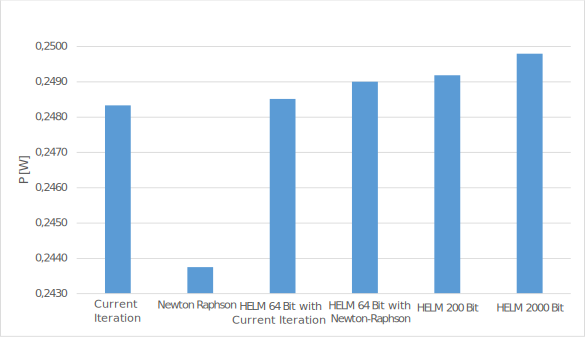
\includegraphics[scale=0.7]{figures/convergence_border}
	\caption{Convergence border for \figinref{convergence_border_net}}
	\label{fig:convergence_border}
\end{figure}

To be able to evaluate \emph{HELM} in detail, also for critical nets, which can not be calculated with the iterative methods, I decided to implement \emph{HELM} with the possibility of a configurable precise datatype. As the generics in \emph{C\#} did not gave me the ability to use a library of precise datatypes together with a package for linear algebra, I decided to switch for this part of the application to \emph{C++}. In this language I had templates available, which allowed the combination of \emph{MPIR} \footnote{http://mpir.org/}, a library for multi precision integers and rationals, with a library for sparse linear algebra, like \emph{Eigen} \footnote{http://eigen.tuxfamily.org/}.

\subsection{Linear Algebra}
All the implemented methods have one thing in common: linear algebra. In all these methods it is necessary to solve linear equation systems, although the equation systems differ in their properties. In \emph{HELM} and the \emph{Current Iteration} the system matrix is the admittance matrix, in \emph{Newton-Raphson} and \emph{FDLF} it is a Jacobian matrix. Both types of matrices are typically sparse, therefore the use of sparse linear algebra improves the performance of the algorithms significantly.

To solve these linear equation systems with a LU-factorization is for big power net quite slow. One possible  solution for this problem is the use of iterative solvers like \emph{BiCGSTAB} \cite{bicgstab}.

Unfortunately, admittance matrices of power nets are sometimes quite bad conditioned, therefore these iterative solvers may not converge to an accurate enough result. To be able to handle these power nets too, it is necessary to reduce the bandwidth of the admittance matrix, for instance through Cuthill-McKee \cite{cuthill}. This reduces the overhead caused by fill-ins during the LU-factorization. Consequently, the memory usage as well as the total runtime is reduced significantly and it is again possible to use the LU-factorization for nets with a six digit number of nodes.

The last important detail of the implementation of the calculation methods is the preconditioning. With this step special properties of the system matrix can be leveraged to improve the condition of the equation system and therefore accelerate the iterative solvers. Fortunately, the admittance matrix, which is the system matrix in the \emph{Current Iteration} and \emph{HELM}, is approximately diagonal dominant. This makes the application of a diagonal preconditioner very practical, because such a preconditioning is very efficient to calculate and improves the condition of the equation system significantly in this special case.

\subsubsection{Optimizations}
The application of the special conditions in \emph{HELM} allows a few optimizations, which can not be made in general. At the beginning I used \emph{Eigen} for the linear algebra, but with bigger power nets I ran into performance problems with this general purpose library. Consequently, I reimplemented the necessary data structures and algorithms:
\begin{itemize}
	\item Dense vector
	\item Sparse matrix
	\item Multiplication of a sparse matrix with a dense vector
	\item Various operations on dense vectors
	\item \emph{BiCGSTAB}
	\item LU-factorization
	\item Forward and back substitution
\end{itemize}

The specialization on dense vectors is useful in the case of \emph{HELM} as the solutions for the equation system will be typically dense. Therefore, there is no need to apply more complex operations on sparse vectors.

However, the system matrix of the linear equation system is the admittance matrix, which is sparse for big problems. In fact, the amount of nonzero values in every row is nearly independent of the size of the total matrix. The reason for this lies within the physical structure of a power net, where every node only as a limited number of neighbours, no matter how big the total graph is. Therefore, the density of the admittance matrix decreases with a growing problem size. For small problems this specialization is in fact a performance drawback, but for these problems the performance does not matter anyway.

As there must not be a zero-row, a version of a sparse matrix with one array for each row is superior over CRS \cite{sparseMatricesJava} or CCS \cite{sparseMatricesJava}. Through this decision regarding the internal representation of the sparse matrix, it is especially during the calculation of the LU-decomposition possible to avoid a lot of memory reallocations, which become the most expensive operations if the sparse matrix is represented internally as CRS or CCS. The decision to store the matrices row- and not column-oriented is related to the matrix multiplication and the forward and back substitution, which benefit in terms of runtime from this format.

The multiplication of a sparse matrix with a dense vector can then leverage the special sparse matrix format and the dense vectors. The key point is to iterate only over the nonzero elements over each row in the matrix and select the according elements of the vector in $\mathcal O(1)$. Additionally, the operation can be parallelized effectively, as all elements in the result vector are independent from each other.

Operations on the dense vectors, like the dot product or adding two vector, can be parallelized too. In this case the dense storage of the values is again very convenient, regarding the performance of the operations.

The iterative solver \emph{BiCGSTAB} benefits from the already optimized matrix and vector operations. Additionally, it is possible to avoid a few memory allocations and move operations through implementing all these operations in-place.

The calculation of a LU-factorization and the forward and back subsitution can not benefit from multiple cores well, at least for small datatypes like a double, where the floating point operations are not that expensive. For bigger datatypes with more expensive operations there is also a small speedup possible.

Last but not least I had also to concentrate on numerical stability. For this purpose, I sorted all values in ascending order before I summed them up. This special modification has of course a negative impact on the performance, but improves the convergence behaviour of \emph{HELM}.

\section{Link to PSS SINCAL}
\label{sec:link_sincal}
The tool developed during this thesis has a parser for the file format of \emph{PSS SINCAL}. This parser allows to read a power net from the file and write back the calculated node voltages.

The basic structure of a power net in \emph{PSS SINCAL} is as follows:
\begin{itemize}
	\item {\textlangle}name{\textrangle}.sin
	\item {\textlangle}name{\textrangle\_}files
	\begin{itemize}
		\item database.001.dia
		\item database.ini
		\item database.mdb
	\end{itemize}
\end{itemize}

The main information about the electrical characteristics of the power net are stored in a database, for instance a \emph{MS Access}-database. It is also possible to use for this a \emph{Oracle Database} or \emph{MS SQL Server}, but as the nets I used during this thesis had a \emph{MS Access}-database beneath I implemented only a parser for this configuration.

Fortunately, this database is documented very well \mbox{online \footnote{http://sincal.s3.amazonaws.com/doc/Misc/SINCAL\_Datenbankinterface.pdf}} and by the documents delivered together with the application.

The most important tables in this database are:
\begin{itemize}
	\item Terminal: contains information about the connection of the net elements with the nodes
	\item VoltageLevel: mostly used for the frequency of the power net
	\item Element: contains all net elements
	\item Node: contains all nodes with their ID, name, voltage level, ... etc.
	\item TwoWindingTransformer, ThreeWindingTransformer, Line, SynchronousMachine, Load, Infeeder: contain the corresponding net elements
	\item LFNodeResult: contains the node results of the load-flow calculation
\end{itemize}

Of course, \emph{PSS SINCAL} supports a lot more net elements and ways to describe than the tool developed during this thesis. Therefore, for more complex or exotic selections in the database the tool will fail to parse the power net. Especially unsymmetric power nets and short circuit calculations are not supported by my tool. Consequently, the tool neglects the values related to these calculations.

For more detailed information about the database I would like to refer to the official documentation, or the implementation of the parser in the subsystem \emph{SincalConnector}. This part of the software has also a few unit tests, which may be used as documentation too.	
	\chapter{Results}
\label{sec:results}
The most interesting questions regarding \emph{HELM} are
\begin{itemize}
	\item How well does \emph{HELM} perform in comparison to the iterative methods?
	\item Is \emph{HELM} able to calculate large scale power nets, for which the iterative methods do not converge?
\end{itemize}
To answer these questions I have run several experiments. The ones related to the first question can be found in \secinref{comparison_algorithms}. To answer the second question I will describe the results of running \emph{HELM} on a large scale power net with a few thousand nodes in \secinref{large_scale_power nets}.

\section{Comparison of the Load-flow Algorithms}
\label{sec:comparison_algorithms}

\begin{table}
	\centering
	\small
	\begin{tabularx}{\textwidth}{|X|p{0.9cm}|p{0.8cm}|p{0.9cm}|p{0.8cm}|p{1.3cm}|}
		\hline
		method & \rotatebox[origin=c]{90}{target precision} & \rotatebox[origin=c]{90}{maximum iterations} & \rotatebox[origin=c]{90}{datatype size} & \rotatebox[origin=c]{90}{maximum coefficients} & \rotatebox[origin=c]{90}{solver} \\ \hline
		\emph{Current Iteration} & 1e-5 & 100 & & & iterative \\ \hline
		\emph{Newton-Raphson} & 1e-5 & 100 & & & iterative \\ \hline
		\emph{HELM} 64-bit & 1e-5 & & 64 & 50 & iterative \\ \hline
		\emph{HELM} 200-bit & 1e-5 & & 200 & 100 & iterative \\ \hline
		\emph{HELM} 64-bit with \emph{Current \mbox{Iteration}} & 1e-5 & 100 & 64 & 50 & iterative \\ \hline
	\end{tabularx}
	\caption{Algorithm parameters for the runtime and accuracy comparison}
	\label{tab:comparison_parameter}
\end{table}

\begin{table}
	\centering
	\small
	\begin{tabularx}{\textwidth}{|X|p{0.9cm}|p{0.8cm}|p{0.9cm}|p{0.8cm}|p{1.3cm}|}
		\hline
		method & \rotatebox[origin=c]{90}{target precision} & \rotatebox[origin=c]{90}{maximum iterations} & \rotatebox[origin=c]{90}{datatype size} & \rotatebox[origin=c]{90}{maximum coefficients} & \rotatebox[origin=c]{90}{solver} \\ \hline
		\emph{HELM}, 64-bit, iterative & 1e-10 & & 64 & 50 & iterative \\ \hline
		\emph{HELM}, 64-bit, LU & 1e-10 & & 64 & 50 & LU \\ \hline
		\emph{HELM} with \emph{Current Iteration}, 64-bit, LU & 1e-10 & 100 & 64 & 50 & LU \\ \hline
		\emph{HELM}, 100-bit, LU & 1e-10 & & 100 & 70 & LU \\ \hline
		\emph{HELM}, 200-bit, LU & 1e-10 & & 200 & 100 & LU \\ \hline
		\emph{HELM}, 1000-bit, LU & 1e-10 & & 1000 & 200 & LU \\ \hline
		\emph{HELM}, 10000-bit, LU & 1e-10 & & 10000 & 300 & LU \\ \hline
		\emph{Current Iteration}, iterative & 1e-10 & 100 & & & iterative \\ \hline
		\emph{Current Iteration}, LU & 1e-10 & 100 & & & LU \\ \hline
		\emph{Newton-Raphson}, iterative & 1e-10 & 100 & & & iterative \\ \hline
		\emph{Newton-Raphson}, LU & 1e-10 & 100 & & & LU \\ \hline
		\emph{Newton-Raphson}, SINCAL & 1e-10 & 100 & & & \\ \hline
	\end{tabularx}
	\caption{Algorithm parameters for the convergence comparison}
	\label{tab:comparison2_parameter}
\end{table}

\begin{figure}
	\centering
	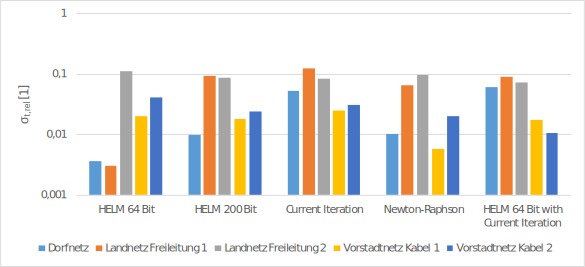
\includegraphics[scale=0.7]{figures/comparison_deviation}
	\caption[Comparison, relative standard deviation of runtime]{Relative standard deviation of the runtime of the algorithms}
	\label{fig:comparison_deviation}
\end{figure}

To compare the different load-flow algorithms I used the sample nets of the Institute and compared the algorithms regarding their runtime and accuracy. I have already considered the improved convergence behaviour in \secinref{implementation_helm}, but I will show additional results regarding this aspect in this chapter.

The selected algorithms for this comparison cover nearly the whole possible spectrum which is implemented in the tool, including the usage of \emph{HELM} to calculate seed values for an iterative method. This special application of \emph{HELM} is represented by the algorithm \emph{HELM} with \emph{Current Iteration}.

The parameters for the algorithms in the accuracy and runtime comparison can be found in \tabinref{comparison_parameter}, the settings for the convergence border tests are in \tabinref{comparison2_parameter}.

To eliminate influences by other processes or the garbage collection at runtime, I ran the calculations five times. The resulting runtimes did not vary much considering the relative standard deviations \figref{comparison_deviation}.

\subsection{Runtime}

\begin{figure}
	\centering
	
\includegraphics[scale=0.7]{figures/comparison_runtime}
	\caption[Comparison, average runtime]{Average runtime of the algorithms for several power nets}
	\label{fig:comparison_runtime}
\end{figure}

One key point is the runtime, and this not only depends on the algorithms themselves, but also on the used tools like the library for the sparse linear algebra. Therefore, I am not able to make absolute statements, especially because I implemented \emph{HELM} in a different language than the other algorithms and optimized the linear algebra in \emph{HELM}.

The first important message here is that \emph{HELM} with 64 bit is considerably fast compared to the \emph{Current Iteration} and \emph{Newton-Raphson}, as seen in \figinref{comparison_runtime}. If \emph{Newton-Raphson} runs into convergence problems like in the case of the \emph{Vorstadtnetz}, \emph{HELM} is even faster than this iterative approach. 

Another conclusion from these tests is that the combination of \emph{HELM} with an iterative method, for instance with the \emph{Current Iteration}, is very useful. In \secinref{implementation_helm} I have already shown that this improves the convergence behaviour, but if we take the runtime into account the combination is not really a drawback. Considering this, I recommend to \emph{always} use \emph{HELM} with the \emph{Current Iteration} instead of only the latter one.

The last important message is the insufficient performance of \emph{HELM} with a datatype bigger than 64 bit. This setting avoids that floating point operations can be executed within a few clock cycles with the integrated assembler commands and therefore degrades the performance of the algorithm significantly. Consequently, I recommend to use \emph{HELM} with a bigger datatype only in situations where the calculation with \emph{HELM} with 64 bit failed.

\subsection{Accuracy}

As an accuracy metric I used the relative power error, which is the ratio between power error and total power, both summed up absolutely:
\begin{equation}
	\epsilon_r = \frac{\sum |P_i - P_{spec,i}| + \sum |Q_i - Q_{spec,i}|}{\sum |P_{spec,i}| + \sum |Q_{spec,i}|}
\end{equation}

The accuracies of the algorithms \figref{comparison_accuracy} were all sufficient for most applications, although a difference can be seen between pure iterative approaches and the ones with \emph{HELM}. The latter ones are able to deliver more accurate results for these nets. Keeping in mind that \emph{HELM} is even as fast as the \emph{Current Iteration}, there is no reason to use the \emph{Current Iteration} instead of \emph{HELM}. Also, \emph{HELM} together with the \emph{Current Iteration} produces more accurate and reliable results than the \emph{Current Iteration} only.

\begin{figure}
	\centering
	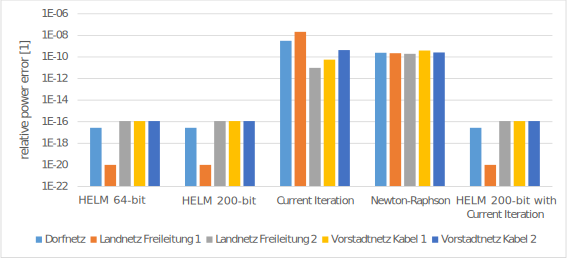
\includegraphics[scale=0.7]{figures/comparison_accuracy}
	\caption[Comparison, accuracy]{Relative power error of the algorithms}
	\label{fig:comparison_accuracy}
\end{figure}

\subsection{Convergence}

To test and compare the convergence behaviour of the different algorithms I used one of the example nets from the Institute, the so-called \emph{Vorstadtnetz}. In this net I increased the load at the most outer ends of the radial net up to that point, where the algorithm did not converge anymore. To find this convergence border more efficiently, I applied the bisection method.

The first and most obvious conclusion, which can be drawn from \figinref{comparison_convergence_border_1}, is that the iterative solver for the internal linear equation systems deteriorates the convergence behaviour of \emph{HELM} significantly. 

Secondly, at least for this special case, the implementation of \emph{Newton-Raphson} in \emph{SINCAL} has a worse convergence behaviour with these settings, compared to my implementation. But I want to make clear that this depends heavily on the settings of the algorithm, and I could only guess how the certain parameters are actually implemented in \emph{SINCAL}. Therefore, it is not really possible to draw a useful conclusion from this experiment regarding the implemention in \emph{SINCAL}.

If we zoom into this chart we get \figinref{comparison_convergence_border_2}, which reveals that \emph{HELM} in its pure form outperforms the other methods, considering the convergence behaviour. After another zoom step one can see in \figinref{comparison_convergence_border_3} that a more accurate datatype improves the convergence behaviour of \emph{HELM}, although only by a few thousand watts. Additionally, such extrordinary settings affect the runtime of the algorithm significantly, as it takes a few hours to calculate such a net, compared to only a few seconds with 64 bit.

\begin{figure}
	\centering
	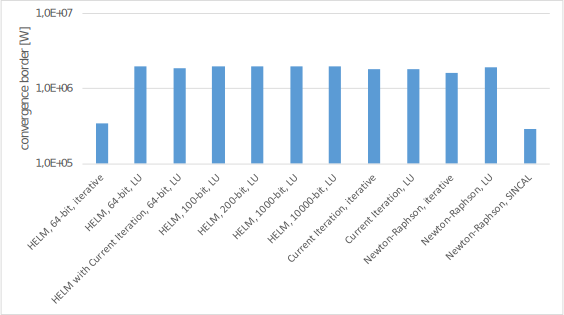
\includegraphics[scale=0.7]{figures/convergence_border_vorstadtnetz_1}
	\caption[Comparison, convergence]{Convergence border of the algorithms}
	\label{fig:comparison_convergence_border_1}
\end{figure}

\begin{figure}
	\centering
	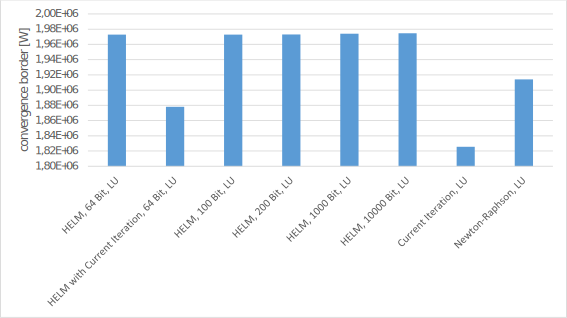
\includegraphics[scale=0.7]{figures/convergence_border_vorstadtnetz_2}
	\caption[Comparison, convergence]{Convergence border of the algorithms}
	\label{fig:comparison_convergence_border_2}
\end{figure}

\begin{figure}
	\centering
	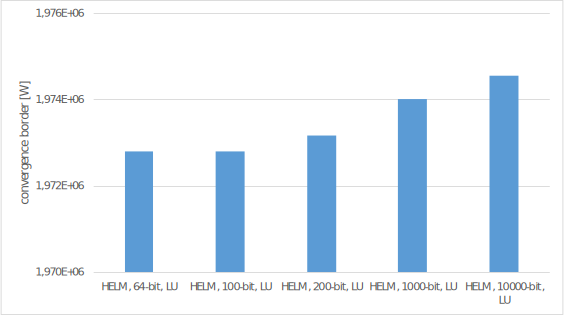
\includegraphics[scale=0.7]{figures/convergence_border_vorstadtnetz_3}
	\caption[Comparison, convergence]{Convergence border of the algorithms}
	\label{fig:comparison_convergence_border_3}
\end{figure}

\section{Calculation of Large-Scale Power Nets}
\label{sec:large_scale_power nets}
	
To evaluate \emph{HELM} in the scenario of large-scale power nets I used the power net of \emph{infra fürth}, which they kindly provided for this purpose. Due to the current limitations of \emph{HELM} I had to adapt the power net. For instance, \emph{HELM} currently does not support non-linear current controlled sources, which were used in the power net of \emph{infra fürth} for the photovoltaic installations, as well as for the generators. To circumvent this I removed all these unsupported elements.

Another important thing to point out is the switching state. The version I received was configured in a way that the total net was split up into three parts. For the comparison later on I used this initial version, as well as one where these three parts were connected together. In the connected version there was one big net with more than 50000 nodes.

As algorithms for the comparison I selected:
\begin{itemize}
	\item \emph{HELM} with a 64 bit datatype and LU factorization
	\item \emph{Current Iteration} with an iterative solver
	\item \emph{HELM} with 64 bit datatype and LU factorization and as second step \emph{Current Iteration} with an iterative solver
	\item \emph{PSS SINCAL} with the default configuration
\end{itemize}
Unfortunately, the library I used for the linear algebra in the iterative load-flow algorithms was not able to calculate the LU factorization in a reasonable amount of time. Additionally, the calculation of the Jacobian matrix was not very efficient either, due to the sparse matrix implementation. Therefore, I had to skip my implementation of \emph{FDLF} and \emph{Newton-Raphson}, but this class of algorithms is still represented in the comparison through \emph{PSS SINCAL}.

As I implemented \emph{HELM} in \emph{C++} and optimized the LU factorization for these circumstances, I was able to select this combination for the tests. This shows that the performance of the algorithms depends heavily on the implementation of the linear algebra.

\begin{figure}
	\centering
	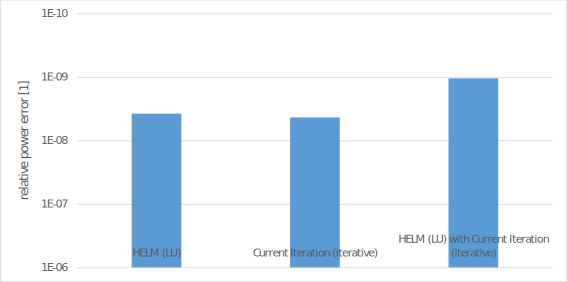
\includegraphics[scale=0.7]{figures/big_net_separate_relative_power_error}
	\caption[Comparison, \emph{infra fürth}, separate, error]{relative power error of the algorithms for the separated version of the power net of \emph{infra fürth}}
	\label{fig:big_net_separate_relative_power_error}
\end{figure}

\begin{figure}
	\centering
	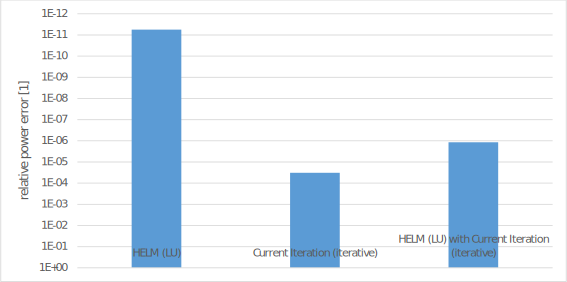
\includegraphics[scale=0.7]{figures/big_net_combined_relative_power_error}
	\caption[Comparison, \emph{infra fürth}, connected, error]{relative power error of the algorithms for the connected version of the power net of \emph{infra fürth}}
	\label{fig:big_net_combined_relative_power_error}
\end{figure}

First, I would like to point out the relative power errors of the algorithms for these two versions of the power net in \figinref{big_net_separate_relative_power_error} and \figinref{big_net_combined_relative_power_error}. For most applications of a load-flow algorithm this accuracy should be sufficient.

\begin{figure}
	\centering
	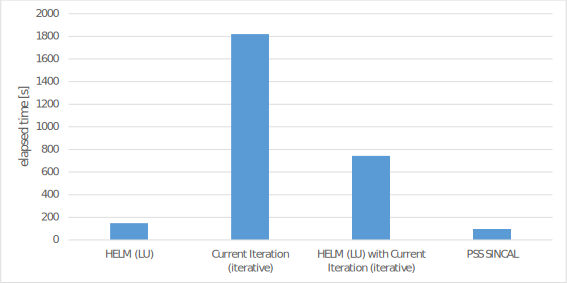
\includegraphics[scale=0.7]{figures/big_net_separate_runtime}
	\caption[Comparison, \emph{infra fürth}, separate, runtime]{runtime of the algorithms for the separated version of the power net of \emph{infra fürth}}
	\label{fig:big_net_separate_runtime}
\end{figure}

\begin{figure}
	\centering
	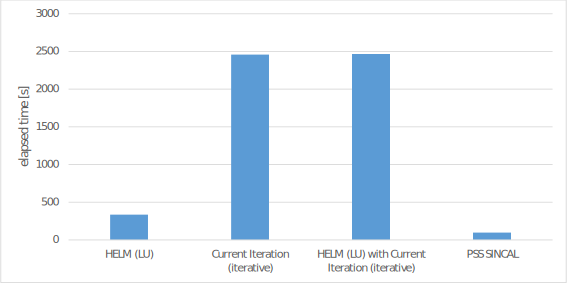
\includegraphics[scale=0.7]{figures/big_net_combined_runtime}
	\caption[Comparison, \emph{infra fürth}, connected, runtime]{runtime of the algorithms for the connected version of the power net of \emph{infra fürth}}
	\label{fig:big_net_combined_runtime}
\end{figure}

Second, the comparison of the runtime in \figinref{big_net_separate_runtime} and \figinref{big_net_combined_runtime} shows that \emph{HELM} is able to get close to the performance of \emph{PSS SINCAL}. Contrary, the \emph{Current Iteration} with the iterative solver for the linear equation systems is outperformed by \emph{HELM} and \emph{PSS SINCAL} by orders of magnitude. Obviously, the main differences is the implementation of the linear algebra, as the admittance matrix is ill-conditioned in these scenarios.

\section{Conclusion}
\emph{HELM} is superior to the iterative methods with regards to the convergence behaviour. This advantage comes directly from the theoretical background, where so far only \emph{HELM} can be proven to have a perfect convergence behaviour. The only limitation which is left here is caused by the machine epsilon of the computer. Considering the runtime, \emph{HELM} can not reach the performance of for instance \emph{FDLF} if the latter one converges within only a few iterations.

In summary, there exist mainly two reasons not to use \emph{HELM}:
\begin{enumerate}
	\item The calculation has to be done fast
	\item A certain control is used in the power net, which is not yet supported by \emph{HELM}
\end{enumerate}
The first drawback here is immanent in \emph{HELM}, but the second one will be a topic for future research.

Finally, in practical applications it is handy to have a fallback in case the iterative methods do not converge.
	
	\cleardoublepage
	\phantomsection
	\listoffigures
	\addcontentsline{toc}{chapter}{\listfigurename}

	\cleardoublepage
	\phantomsection
	\listofequationname
	\addcontentsline{toc}{chapter}{\listequationsname}

	\cleardoublepage	
	\begin{thebibliography}{1}
		\bibitem{helmIEEE}
		A.~Trias, \emph{The Holomorphic Embedding Load Flow Method}, IEEE PES General Meeting, July 2012
		
		\bibitem{helmPV}
		M.~K.~Subramanian, Y.~Feng, D.~Tylavsky, \emph{PV Bus Modeling in a Holomorphically Embedded Power-Flow Formulation}, 978-1-4799-1255-1/13, IEEE, 2013
		
		\bibitem{helmPatentApr2009}
		A.~Trias, \emph{System and Method for Monitoring and Managing Electrical Power Transmission and Distribution Networks}, US Patent 7,519,506 B2, April 2009
		
		\bibitem{helmPatentSept2009}
		A.~Trias, \emph{System and Method for Monitoring and Managing Electrical Power Transmission and Distribution Networks}, US Patent US 2009/0228154 A1, September 2009
					
		\bibitem{epsilonWynn}
		P.~Wynn, \emph{The Epsilon Algorithm and Operational Formulas of Numerical Analysis}, June 1960
		
	\end{thebibliography}
\end{document}